\documentclass[11pt,letterpaper]{article}
\usepackage[lmargin=1in,rmargin=1in,tmargin=1in,bmargin=1in]{geometry}
\usepackage{../style/homework}
\usepackage{../style/commands}
\setbool{quotetype}{true} % True: Side; False: Under
\setbool{hideans}{false} % Student: True; Instructor: False

% -------------------
% Content
% -------------------
\begin{document}

\homework{18: Due 12/11}{Go down deep enough into anything and you will find Mathematics.}{Dean Schlicter}

% Problem 1
\problem{10} Consider the polynomial $f(x)= (x - 1)(x + 3)(x^2 + 4)(x^2 - 9)$. 
	\begin{enumerate}[(a)]
	\item What is the degree of $f(x)$?
	\item How many real zeros does $f(x)$ have?
	\item How many complex zeros does $f(x)$ have?
	\item Does $f(x)$ have a maximum or a minimum? Explain. 
	\end{enumerate} \pspace

\sol
\begin{enumerate}[(a)]
\item The degree of $p_1(x) p_2(x) \cdots p_m(x)$, where the $p_i(x)$ are polynomials, are is the sum of the degrees of the $p_i(x)$. But then the degree of $f(x)$ is $1 + 1 + 2 + 2= 6$. \pspace

\item Setting $f(x)= 0$, we have $(x - 1)(x + 3)(x^2 + 4)(x^2 - 9)= 0$. But then either $x - 1= 0$, which implies $x= 1$ or $x + 3= 0$, which implies $x= -3$ or $x^2 + 4= 0$, which implies $x^2= -4$ (which is impossible for real numbers, so this has only complex zeros) or $x^2 - 9= 0$. Now $x^2 - 9= (x - 3)(x + 3)$---being the difference of perfect squares. But then $x^2 - 9= 0$ implies that $(x - 3)(x + 3)= 0$. This means either $x - 3= 0$, which implies $x= 3$ or $x + 3= 0$, which implies $x= -3$. Therefore, $f(x)$ has $1 + 1 + 2= 4$ real zeros. \pspace

\item From (b), we see the complex zeros of $f(x)$ `come from' the $x^2 + 4$ term. If $x^2 + 4= 0$, then $x^2= -4$. But then $x= \sqrt{-4}= \pm \sqrt{4} i= \pm 2i$. Therefore, $f(x)$ has two complex zeros. \pspace

\item From (a), we know the degree of $f(x)$ is 6---which is even. Therefore, the `ends' of $f(x)$ point in the same `direction.' But then $f(x)$ has either has a maximum, if $a < 0$ and $f(x)$ opens `downwards', or a minimum, if $a > 0$ and $f(x)$ opens `upwards.' The leading coefficient is the product of the leading coefficients of the terms of $f(x)$. Therefore, the leading coefficient of $f(x)$ is $1 \cdot 1 \cdot 1 \cdot 1= 1 > 0$. Therefore, $f(x)$ opens `upwards' so that $f(x)$ has a minimum value but will not have a maximum value. 
\end{enumerate}



\newpage



% Problem 2
\problem{10} Determine the quadratic polynomial that has a root at $x= 1 - 3i$ and has $y$-intercept 5. \pspace

\sol For a quadratic polynomial to be real, the complex roots must come in complex conjugate pairs. Therefore, if $1 - 3i$ is a root for the polynomial, $\overline{1 - 3i}= 1 + 3i$ must be a root of the polynomial. Because a quadratic polynomial has degree two (by definition), it must have exactly two roots (counting complex roots and counting roots with multiplicity) by the Fundamental Theorem of Algebra. Because we have two roots, namely $1 \pm 3i$, these must be all the roots of the polynomial. But then the polynomial must have the form\dots
	\[
	\begin{gathered}
	A \big(x - (1 - 3i) \big) \big(x - (1 + 3i) \big) \\[0.3cm]
	A (x^2 - x(1 + 3i) - x(1 - 3i) + (1 - 3i)(1 + 3i) \big) \\[0.3cm]
	A \big(x^2 - x - 3ix - x + 3ix + (1 + 3i - 3i - 9i^2) \big) \\[0.3cm]
	A \big(x^2 - 2x - 1 + 9(-1) \big) \\[0.3cm]
	A(x^2 - 2x - 10) 
	\end{gathered}
	\]  \pspace
We know this polynomial must have $y$-intercept of 5; that is, $y= 5$ when $x= 0$. But then\dots
	\[
	\begin{gathered}
	5= A(0^2 - 2(0) - 10) \\
	5= -10A \\
	A= -\dfrac{5}{10} \\
	A= -\dfrac{1}{2}
	\end{gathered}
	\] \pspace
Therefore, it must be that the polynomial is\dots
	\[
	-\dfrac{1}{2} (x^2 - 2x - 10)
	\]



\newpage



% Problem 3
\problem{10} Suppose that $f(x)$ is a degree four polynomial (quartic polynomial) with $f(-3)= f(1)= f(4)= f(6)= 0$ and $f(0)= -7$. Find the polynomial $f(x)$. \pspace

\sol Because $f(-3)= 0$, $f(1)= 0$, $f(4)= 0$, and $f(6)= 0$, we know that $f(x)$ has zeros $-3$, $1$, $4$, and $6$. Therefore, $f(x)$ has the form $A \big(x - (-3) \big)^{n_1} (x - 1)^{n_2} (x - 4)^{n_3} (x - 6)^{n_4}$ for some integers $n_1, n_2, n_3, n_4 \geq 1$. The degree of $f(x)$ is thus far $n_1 + n_2 + n_3 + n_4$. Because $f(x)$ has degree 4, we know that $n_1 + n_2 + n_3 + n_4= 4$. Because each of the $n_i$ is at least 1, it must be that $n_1= n_2= n_3= n_4= 1$. Therefore, 
	\[
	f(x)= A (x + 3)(x - 1)(x - 4)(x - 6)
	\] \pspace
But we know that $f(0)= -7$. Therefore, we have\dots
	\[
	\begin{gathered}
	f(0)= A(0 + 3)(0 - 1)(0 - 4)(0 - 6) \\[0.3cm]
	-7= A(3)(-1)(-4)(-6) \\[0.3cm]
	-7= -72A \\[0.3cm]
	A= \dfrac{7}{72}
	\end{gathered}
	\]
Therefore, we know that\dots
	\[
	f(x)= \dfrac{7}{72}\, (x + 3)(x - 1)(x - 4)(x - 6)
	\]



\newpage



% Problem 4
\problem{10} Suppose $f(x)$ is a real quartic polynomial whose graph is given below. How many real zeros does $f(x)$ have? How many complex zeros does $f(x)$ have? Find $f(x)$. 
	\[
	\fbox{
	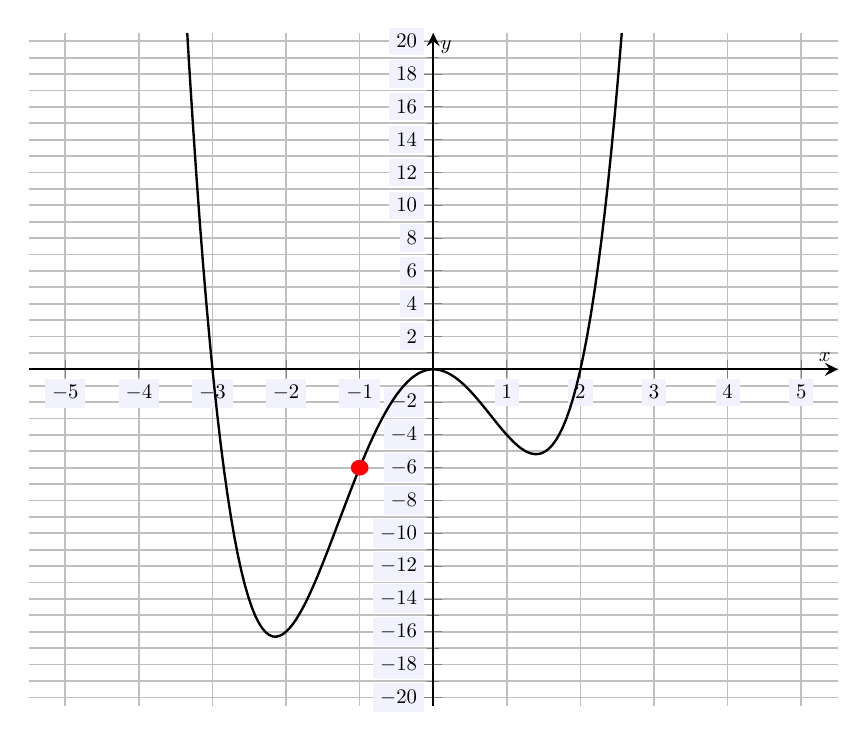
\begin{tikzpicture}[scale=1.5,every node/.style={scale=0.5}]
	\begin{axis}[
	grid=both,
	axis lines=middle,
	ticklabel style={fill=blue!5!white},
	xmin= -5.5, xmax=5.5,
	ymin= -20.5, ymax=20.5,
	xtick={-5,-4,...,5},
	ytick={-20,-18,...,20},
	minor tick = {-20,-19,...,20},
	xlabel=\(x\),ylabel=\(y\),
	]
	\addplot[line width= 0.02cm,samples=150,domain= -3.5:3.5] ({x},{x*x*(x - 2)*(x + 3)});
	\draw[draw=none,fill=red] (-1,-6) circle (0.12 and 0.48);
	\end{axis}
	\end{tikzpicture}
	}
	\] \pspace

\sol From the graph of $f(x)$, we can see that $x= -3$, $x= 0$, and $x= 2$ must be zeros of $f(x)$. Furthermore, because the zero at $x= 0$ intersects the $x$-axis `tangentially', the multiplicity of $x= 0$ must be at least 2. But then $f(x)$ must have degree at least $1 + 2 + 1= 4$. Because $f(x)$ is quartic, it has degree 4. Therefore, $f(x)$ cannot have any complex roots. So we know $f(x)$ has the form\dots
	\[
	f(x)= A \big(x - (-3) \big) (x - 0)^2 (x - 2)= A x^2(x + 3)(x - 2)
	\]
We can see that $(-1, -6)$ is a point on the graph of $f(x)$; that is, $f(-1)= -6$. But then\dots
	\[
	\begin{gathered}
	f(x)= A x^2(x + 3)(x - 2) \\[0.3cm]
	f(-1)= A (-1)^2 (-1 + 3)(-1 - 2) \\[0.3cm]
	-6= A \cdot 1(2)(-3) \\[0.3cm]
	-6= -6A \\[0.3cm]
	A= 1
	\end{gathered}
	\]
Therefore, we must have\dots
	\[
	f(x)= x^2(x + 3)(x - 2)
	\]


\end{document}